\documentclass[a4paper,oneside,DIV=12,12pt]{scrartcl}

\usepackage{graphicx}
\usepackage{float}

\usepackage{fontspec}
\setmainfont{STIX Two Text}
%\setsansfont{Roboto}
\newfontfamily{\cyrillicfontsf}{Roboto}

\usepackage{microtype}

\usepackage{polyglossia}
\setmainlanguage{ukrainian}

\usepackage{amsmath}
\usepackage{unicode-math}
\setmathfont{STIX Two Math}

\usepackage{IEEEtrantools}

\usepackage{karnaugh-map}

\usepackage{booktabs}

\usepackage{tikz}
\usetikzlibrary{arrows,automata,positioning}

\usepackage{siunitx}
\sisetup{output-decimal-marker = {,},
exponent-product = {\cdot}}

% Problem-solution typesetting
\usepackage{xsim}
\loadxsimstyle{runin}
\DeclareExerciseTranslations{exercise}{
	Ukrainian	=	завдання ,
}

\DeclareExerciseTranslations{solution}{
	Ukrainian	=	розв'язання ,
}

\xsimsetup{
	solution/print = true,
	exercise/template = runin,
	solution/template = runin,
}

\renewcommand{\implies}{\rightarrow}

\newcommand\barneg[1]{\overline{#1}}
\newcommand{\logicequiv}{\leftrightarrow}

\begin{document}
	\begin{titlepage}
		\begin{center}
			Міністерство освіти і науки України\\
			Національний авіаційний університет\\
			Навчально-науковий інститут комп'ютерних інформаційних технологій\\
			Кафедра комп'ютеризованих систем управління
			
			\vspace{\fill}
				Академічна різниця\\
				з дисципліни:\\
				«Комп'ютерна логіка»\\
				I семестр
				
			\vspace{\fill}
			
			\begin{flushright}
				Виконав:\\
				студент ННІКІТ СП-225\\
				Клокун Владислав\\
			\end{flushright}
			Київ 2017
		\end{center}
	\end{titlepage}
	
	\begin{exercise}
		Опишіть логічні (булеві) функції від двох змінних.
	\end{exercise}
	
	\begin{solution}
		Булева функція від двох змінних --- це відображення $B^2 \mapsto B$, де $B = \{0, 1\}$. Для двох аргументів існує $2^{2^2} = 16$ можливих булевих функцій. Однак, найчастіше використовуються лише декілька. Розглянемо їх за допомогою таблиці істинності.
		
		\begin{table}[!htbp]
		\centering
			\begin{tabular}{cccccc}
				\toprule
					    % &     & НЕ           & І & АБО \\
					$x$ & $y$ & $\neg{x}$ & $x \land y$ & $x \lor y$ & $x \implies y$ \\
				\midrule
					0   & 0   & 1            & 0           & 0          & 1 \\
					0   & 1   & 1            & 0           & 1          & 1 \\
					1   & 0   & 0            & 0           & 1          & 0 \\
					1   & 1   & 0            & 1           & 1          & 1 \\
				\bottomrule
			\end{tabular}
		\caption{Таблиця істинності основних булевих функцій}
		\label{fig:bool-functioins-truth-table}
		\end{table}
	\end{solution}
	
	\begin{exercise}
		Побудувати таблицю істинності для функції $F$:
		\[
			F(x, y, z) = \left( \neg{(xy)} \implies z\right) \logicequiv \left( x \neg{z} \implies y \right).
		\]
	\end{exercise}
	
	\begin{solution}
		Таблиця істинності заданої функції наведена у табл.~\ref{tab:ex2-truth-table}.
		
		\begin{table}[!htbp]
		\centering
			\begin{tabular}{cccc}
				\toprule
					$x$ & $y$ & $z$ & $F(x, y, z)$\\
				\midrule
					0   & 0   & 0   & 0\\
					0   & 0   & 1   & 1\\
					0   & 1   & 0   & 1\\
					0   & 1   & 1   & 1\\
					1   & 0   & 0   & 0\\
					1   & 0   & 1   & 1\\
					1   & 1   & 0   & 1\\
					1   & 1   & 1   & 1\\
				\bottomrule
			\end{tabular}
		\caption{Таблиця істинності заданої функції}
		\label{tab:ex2-truth-table}
		\end{table}
	\end{solution}
	
	\begin{exercise}
		Виконайте спрощення логічного виразу
		\[
			L = x_3x_2 \lor x_3 \barneg{x_2} \lor \barneg{\barneg{x_1} \lor \barneg{x_1 \lor x_2} }.
		\]
		Виконайте мінімізацію логічного виразу
		\[
			F = 0 \lor 4 \lor 7 \lor 8 \lor 11 \lor 12 \lor 13 \lor 15.
		\]
	\end{exercise}
	
	\begin{solution}
		Спростимо логічний вираз $L$, використовуючи закони Де~Моргана, подвійного заперечення, ідемпотенції та дистрибутивності.
		\begin{IEEEeqnarray*}{rCl}
			%L &=& x_3x_2 \lor x_3 \barneg{x_2} \lor \barneg{\barneg{x_1} \lor \barneg{x_1 \lor x_2} }\\
			%  &=& x_3 x_2 \lor x_3 \barneg{x_2} \lor \barneg{\barneg{x_1}} \barneg{\barneg{(x_1 \lor x_2)}}\\
			%  &=& x_3 x_2 \lor x_3 \barneg{x_2} \lor x_1 x_1 \lor x_2\\
			%  &=& x_3 x_2 \lor x_3 \barneg{x_2} \lor x_1 x_1 \lor x_1 x_2\\
			%  &=& x_3 (x_2 \lor \barneg{x_2}) \lor x_1 \lor x_1 x_2\\
			%  &=& x_3 \lor x_2 \lor x_1(1 + x_2)\\
			%  &=& x_3 \lor x_1.
			%  
			L &=& x_3 \land x_2 \lor x_3 \land \neg x_2 \lor \neg (\neg x_1 \lor \neg(x_1 \lor x_2)\\
			  &=& x_3 \land x_2 \lor x_3 \land \neg x_2 \lor \neg (\neg x_1) \land \neg(\neg (x_1 \lor x_2))\\
			  &=& x_3 \land x_2 \lor x_3 \land \neg x_2 \lor x_1 \land (x_1 \lor x_2)\\
			  &=& x_3 \land x_2 \lor x_3 \land \neg x_2 \lor x_1 \land x_1 \lor x_1 \land x_2\\
			  &=& x_3 \land (x_2 \lor \neg x_2) \lor x_1 \lor x_1 \land x_2\\
			  &=& x_3 \lor x_1 \lor x_1 \land x_2\\
			  &=& x_3 \lor x_1 \land (1 \lor x_2)\\
			  &=& x_3 \lor x_1.
		\end{IEEEeqnarray*}
		
		Мінімізуємо логічний вираз $F$. Для цього представимо його у двійковому вигляді:
		\begin{IEEEeqnarray*}{rCl}
			F &=& 0 \lor 4 \lor 7 \lor 8 \lor 11 \lor 12 \lor 13 \lor 15\\
			  &=& 0000 \lor 0100 \lor 0111 \lor 1000 \lor 1011 \lor 1100 \lor 1101 \lor 1111\\
			  &=& \neg{A} \neg{B} \neg{C} \neg{D}
			      \lor \neg{A}      B \neg{C} \neg{D}
			      \lor \neg{A}      B  \neg{C} \neg{D}
			      \lor \neg{A}      B       C       D \\
			  &&  \lor      A  \neg{B} \neg{C} \neg{D}
			      \lor      A  \neg{B}      C       D
			      \lor      A       B  \neg{C}      D
			      \lor      A       B       C       D
		\end{IEEEeqnarray*}
		
		Побудуємо карту Карно (рис.~\ref{fig:task2-karnaugh-map}).
		\begin{figure}
		\centering
			\begin{karnaugh-map}*[4][4][1][$CD$][$AB$]
				\minterms{0,4,7,8,11,12,13,15}
				\implicant{0}{8}
				\implicant{12}{15}
				\implicant{ 7}{15}
				\implicant{15}{11}
			\end{karnaugh-map}
		\caption{Карта Карно логічного виразу $F$}
		\label{fig:task2-karnaugh-map}
		\end{figure}
		Звідси маємо:
		\[
			F = \neg{C} \neg{D} \lor ABD \lor BCD \lor ACD.
		\]
	\end{solution}
	
	\begin{exercise}
		Отримати МДНФ перемикальної функції, що задана діаграмою Вейча (рис.~\ref{fig:task3-veitch-diagram}). Для мінімізації застосувати метод Квайна~--- МакКласкі. Перемикальну функцію реалізувати в елементному базисі АБО---НЕ.
		
		\begin{figure}[!htbp]
		\centering
			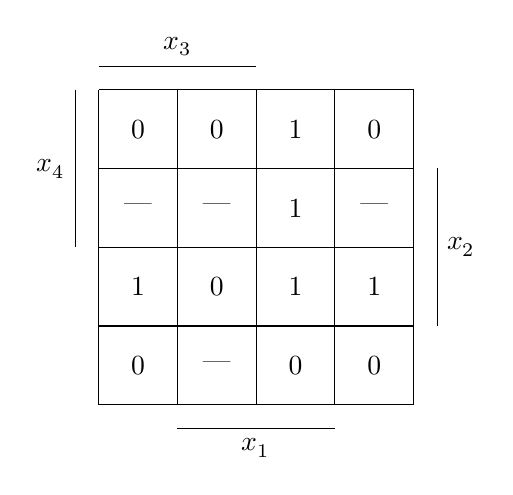
\begin{tikzpicture}
				\draw (0,0) grid (4,4);
				\node at (0.5,0.5){0};
				\node at (1.5,0.5){—};
				\node at (2.5,0.5){0};
				\node at (3.5,0.5){0};

				\node at (0.5,1.5){1};
				\node at (1.5,1.5){0};
				\node at (2.5,1.5){1};
				\node at (3.5,1.5){1};
				
				\node at (0.5,2.5){—};
				\node at (1.5,2.5){—};
				\node at (2.5,2.5){1};
				\node at (3.5,2.5){—};
				
				\node at (0.5,3.5){0};
				\node at (1.5,3.5){0};
				\node at (2.5,3.5){1};
				\node at (3.5,3.5){0};
				
				\draw (0,4.3) --node[midway, above]{$x_3$} (2,4.3);
				\draw (-0.3,4) --node[midway, left]{$x_4$} (-0.3,2);
				\draw (1,-0.3) --node[midway, below]{$x_1$} (3,-0.3);
				\draw (4.3,1) --node[midway, right]{$x_2$} (4.3,3);
			\end{tikzpicture}
		\caption{Діаграма Вейча заданої перемикальної функції}
		\label{fig:task3-veitch-diagram}
		\end{figure}
		
	\end{exercise}
	
	\begin{exercise}
		За даним графом автомата виконати синтез керуючого автомата.
		
		\begin{figure}[!htbp]
		\centering
			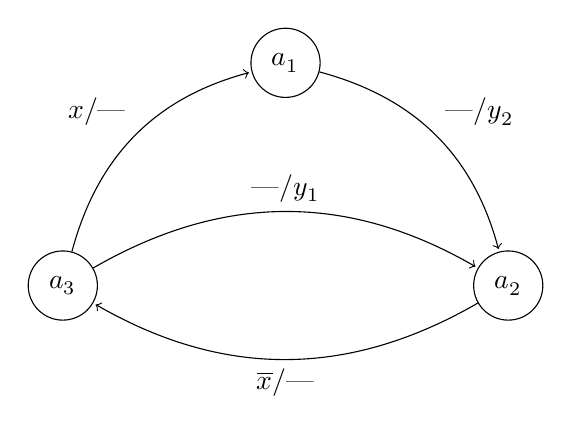
\begin{tikzpicture}[shorten >=1pt,node distance=4cm,on grid,auto]
				
				\node[state]	(a_1)		{$a_1$};
				\node[state]	(a_2) [below right=of a_1]	{$a_2$};
				\node[state]	(a_3) [below left=of a_1]	{$a_3$};
				
				\path[->]	(a_1)	edge [bend left=30]	node {$— / y_2$}	(a_2)
							(a_2)	edge [bend left=30]	node {$\barneg{x} / —$}				(a_3)
							(a_3)	edge [bend left=30]	node {$x / —$}		(a_1)
									edge [bend left=30]	node {$— / y_1$}	(a_2);
				
			\end{tikzpicture}
		\end{figure}
		Для побудови функціональної схеми використати T-тригери. Елементний базис: І, АБО, НЕ.
	\end{exercise}
\end{document}